\documentclass[twoside]{book}

% Packages required by doxygen
\usepackage{fixltx2e}
\usepackage{calc}
\usepackage{doxygen}
\usepackage[export]{adjustbox} % also loads graphicx
\usepackage{graphicx}
\usepackage[utf8]{inputenc}
\usepackage{makeidx}
\usepackage{multicol}
\usepackage{multirow}
\PassOptionsToPackage{warn}{textcomp}
\usepackage{textcomp}
\usepackage[nointegrals]{wasysym}
\usepackage[table]{xcolor}

% Font selection
\usepackage[T1]{fontenc}
\usepackage[scaled=.90]{helvet}
\usepackage{courier}
\usepackage{amssymb}
\usepackage{sectsty}
\renewcommand{\familydefault}{\sfdefault}
\allsectionsfont{%
  \fontseries{bc}\selectfont%
  \color{darkgray}%
}
\renewcommand{\DoxyLabelFont}{%
  \fontseries{bc}\selectfont%
  \color{darkgray}%
}
\newcommand{\+}{\discretionary{\mbox{\scriptsize$\hookleftarrow$}}{}{}}

% Page & text layout
\usepackage{geometry}
\geometry{%
  a4paper,%
  top=2.5cm,%
  bottom=2.5cm,%
  left=2.5cm,%
  right=2.5cm%
}
\tolerance=750
\hfuzz=15pt
\hbadness=750
\setlength{\emergencystretch}{15pt}
\setlength{\parindent}{0cm}
\setlength{\parskip}{3ex plus 2ex minus 2ex}
\makeatletter
\renewcommand{\paragraph}{%
  \@startsection{paragraph}{4}{0ex}{-1.0ex}{1.0ex}{%
    \normalfont\normalsize\bfseries\SS@parafont%
  }%
}
\renewcommand{\subparagraph}{%
  \@startsection{subparagraph}{5}{0ex}{-1.0ex}{1.0ex}{%
    \normalfont\normalsize\bfseries\SS@subparafont%
  }%
}
\makeatother

% Headers & footers
\usepackage{fancyhdr}
\pagestyle{fancyplain}
\fancyhead[LE]{\fancyplain{}{\bfseries\thepage}}
\fancyhead[CE]{\fancyplain{}{}}
\fancyhead[RE]{\fancyplain{}{\bfseries\leftmark}}
\fancyhead[LO]{\fancyplain{}{\bfseries\rightmark}}
\fancyhead[CO]{\fancyplain{}{}}
\fancyhead[RO]{\fancyplain{}{\bfseries\thepage}}
\fancyfoot[LE]{\fancyplain{}{}}
\fancyfoot[CE]{\fancyplain{}{}}
\fancyfoot[RE]{\fancyplain{}{\bfseries\scriptsize Generated by Doxygen }}
\fancyfoot[LO]{\fancyplain{}{\bfseries\scriptsize Generated by Doxygen }}
\fancyfoot[CO]{\fancyplain{}{}}
\fancyfoot[RO]{\fancyplain{}{}}
\renewcommand{\footrulewidth}{0.4pt}
\renewcommand{\chaptermark}[1]{%
  \markboth{#1}{}%
}
\renewcommand{\sectionmark}[1]{%
  \markright{\thesection\ #1}%
}

% Indices & bibliography
\usepackage{natbib}
\usepackage[titles]{tocloft}
\setcounter{tocdepth}{3}
\setcounter{secnumdepth}{5}
\makeindex

% Hyperlinks (required, but should be loaded last)
\usepackage{ifpdf}
\ifpdf
  \usepackage[pdftex,pagebackref=true]{hyperref}
\else
  \usepackage[ps2pdf,pagebackref=true]{hyperref}
\fi
\hypersetup{%
  colorlinks=true,%
  linkcolor=blue,%
  citecolor=blue,%
  unicode%
}

% Custom commands
\newcommand{\clearemptydoublepage}{%
  \newpage{\pagestyle{empty}\cleardoublepage}%
}

\usepackage{caption}
\captionsetup{labelsep=space,justification=centering,font={bf},singlelinecheck=off,skip=4pt,position=top}

%===== C O N T E N T S =====

\begin{document}

% Titlepage & ToC
\hypersetup{pageanchor=false,
             bookmarksnumbered=true,
             pdfencoding=unicode
            }
\pagenumbering{roman}
\begin{titlepage}
\vspace*{7cm}
\begin{center}%
{\Large antiplag }\\
\vspace*{1cm}
{\large Generated by Doxygen 1.8.11}\\
\end{center}
\end{titlepage}
\clearemptydoublepage
\tableofcontents
\clearemptydoublepage
\pagenumbering{arabic}
\hypersetup{pageanchor=true}

%--- Begin generated contents ---
\chapter{Namespace Index}
\section{Namespace List}
Here is a list of all namespaces with brief descriptions:\begin{DoxyCompactList}
\item\contentsline{section}{\hyperlink{namespace_ui}{Ui} }{\pageref{namespace_ui}}{}
\end{DoxyCompactList}

\chapter{Hierarchical Index}
\section{Class Hierarchy}
This inheritance list is sorted roughly, but not completely, alphabetically\+:\begin{DoxyCompactList}
\item \contentsline{section}{Document}{\pageref{class_document}}{}
\item \contentsline{section}{Homework}{\pageref{class_homework}}{}
\item \contentsline{section}{Pattern}{\pageref{class_pattern}}{}
\item \contentsline{section}{Pattern\+Tree}{\pageref{class_pattern_tree}}{}
\item \contentsline{section}{Project}{\pageref{class_project}}{}
\item \contentsline{section}{qt\+\_\+meta\+\_\+stringdata\+\_\+\+Widget\+\_\+t}{\pageref{structqt__meta__stringdata___widget__t}}{}
\item Q\+Widget\begin{DoxyCompactList}
\item \contentsline{section}{Widget}{\pageref{class_widget}}{}
\end{DoxyCompactList}
\item \contentsline{section}{Ui\+\_\+\+Widget}{\pageref{class_ui___widget}}{}
\begin{DoxyCompactList}
\item \contentsline{section}{Ui\+:\+:Widget}{\pageref{class_ui_1_1_widget}}{}
\end{DoxyCompactList}
\end{DoxyCompactList}

\chapter{Class Index}
\section{Class List}
Here are the classes, structs, unions and interfaces with brief descriptions:\begin{DoxyCompactList}
\item\contentsline{section}{\hyperlink{class_document}{Document} }{\pageref{class_document}}{}
\item\contentsline{section}{\hyperlink{class_homework}{Homework} }{\pageref{class_homework}}{}
\item\contentsline{section}{\hyperlink{class_pattern}{Pattern} \\*Storing patterns from a document }{\pageref{class_pattern}}{}
\item\contentsline{section}{\hyperlink{class_pattern_tree}{PatternTree} }{\pageref{class_pattern_tree}}{}
\item\contentsline{section}{\hyperlink{class_project}{Project} }{\pageref{class_project}}{}
\item\contentsline{section}{\hyperlink{structqt__meta__stringdata___widget__t}{qt\_meta\_stringdata\_Widget\_t} }{\pageref{structqt__meta__stringdata___widget__t}}{}
\item\contentsline{section}{\hyperlink{class_ui___widget}{Ui\_Widget} }{\pageref{class_ui___widget}}{}
\item\contentsline{section}{\hyperlink{class_ui_1_1_widget}{Ui::Widget} }{\pageref{class_ui_1_1_widget}}{}
\item\contentsline{section}{\hyperlink{class_widget}{Widget} }{\pageref{class_widget}}{}
\end{DoxyCompactList}

\chapter{Namespace Documentation}
\hypertarget{namespace_ui}{}\section{Ui Namespace Reference}
\label{namespace_ui}\index{Ui@{Ui}}
\subsection*{Classes}
\begin{DoxyCompactItemize}
\item 
class \hyperlink{class_ui_1_1_widget}{Widget}
\end{DoxyCompactItemize}

\chapter{Class Documentation}
\hypertarget{class_document}{}\section{Document Class Reference}
\label{class_document}\index{Document@{Document}}
\subsection*{Public Member Functions}
\begin{DoxyCompactItemize}
\item 
\hyperlink{class_document_ad6f3eb7808d3d6ad6f40e5b64a3317bc}{Document} (std\+::string address)
\item 
void \hyperlink{class_document_a607bc11ebda64c08fd22c8ca7aa373d3}{Rabin\+Karp} ()
\begin{DoxyCompactList}\small\item\em Perform Rabin-\/\+Karp algorithm for this document. \end{DoxyCompactList}\item 
void \hyperlink{class_document_aa02349519b475996d1206dfbbcaab349}{K\+MP} ()
\begin{DoxyCompactList}\small\item\em Perdorm K\+MP algorithm for this document. \end{DoxyCompactList}\item 
std\+::string \hyperlink{class_document_aba3c51ac1b4cb63dd9235aaa9e5ab6f0}{get\+Address} ()
\end{DoxyCompactItemize}
\subsection*{Protected Member Functions}
\begin{DoxyCompactItemize}
\item 
void \hyperlink{class_document_a019a44be44bd7b548ea32e4c699bed49}{make\+Pattern} ()
\begin{DoxyCompactList}\small\item\em Make the patterns with winnowing algorithm. \end{DoxyCompactList}\item 
void \hyperlink{class_document_a508bc7255ec6ddf96d0d7078ff0d1229}{preprocess} ()
\item 
bool \hyperlink{class_document_ae81119fe62cb6c73bff4c9283c97884f}{is\+Valid} (char c)
\end{DoxyCompactItemize}
\subsection*{Private Member Functions}
\begin{DoxyCompactItemize}
\item 
\hyperlink{class_document}{Document} \& \hyperlink{class_document_a4ccdb9185bd311793ad385564553153c}{operator=} (const \hyperlink{class_document}{Document} \&other)
\end{DoxyCompactItemize}
\subsection*{Private Attributes}
\begin{DoxyCompactItemize}
\item 
std\+::string \hyperlink{class_document_a20ece3a3a1e633e381d28813ad76a088}{m\+\_\+address}
\item 
std\+::string \hyperlink{class_document_a7d965b64a228ab63761ec4440a5549e0}{m\+\_\+content}
\item 
std\+::vector$<$ \hyperlink{class_pattern}{Pattern} $>$ \hyperlink{class_document_a6cdddf9610a671723515bb6c71553870}{m\+\_\+patterns}
\end{DoxyCompactItemize}


\subsection{Constructor \& Destructor Documentation}
\index{Document@{Document}!Document@{Document}}
\index{Document@{Document}!Document@{Document}}
\subsubsection[{\texorpdfstring{Document(std\+::string address)}{Document(std::string address)}}]{\setlength{\rightskip}{0pt plus 5cm}Document\+::\+Document (
\begin{DoxyParamCaption}
\item[{std\+::string}]{address}
\end{DoxyParamCaption}
)}\hypertarget{class_document_ad6f3eb7808d3d6ad6f40e5b64a3317bc}{}\label{class_document_ad6f3eb7808d3d6ad6f40e5b64a3317bc}


Here is the call graph for this function\+:\nopagebreak
\begin{figure}[H]
\begin{center}
\leavevmode
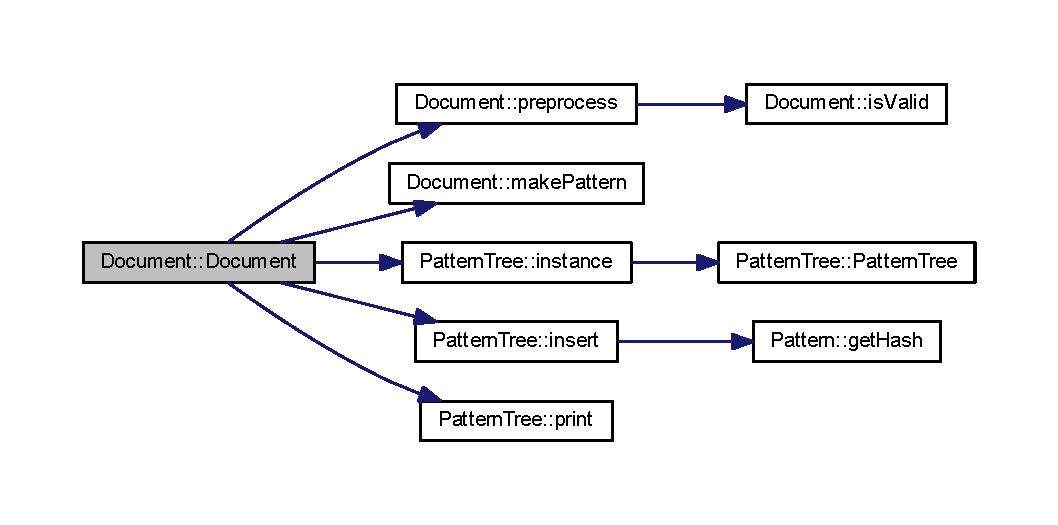
\includegraphics[width=350pt]{class_document_ad6f3eb7808d3d6ad6f40e5b64a3317bc_cgraph}
\end{center}
\end{figure}




\subsection{Member Function Documentation}
\index{Document@{Document}!get\+Address@{get\+Address}}
\index{get\+Address@{get\+Address}!Document@{Document}}
\subsubsection[{\texorpdfstring{get\+Address()}{getAddress()}}]{\setlength{\rightskip}{0pt plus 5cm}std\+::string Document\+::get\+Address (
\begin{DoxyParamCaption}
{}
\end{DoxyParamCaption}
)\hspace{0.3cm}{\ttfamily [inline]}}\hypertarget{class_document_aba3c51ac1b4cb63dd9235aaa9e5ab6f0}{}\label{class_document_aba3c51ac1b4cb63dd9235aaa9e5ab6f0}


Here is the call graph for this function\+:
\nopagebreak
\begin{figure}[H]
\begin{center}
\leavevmode
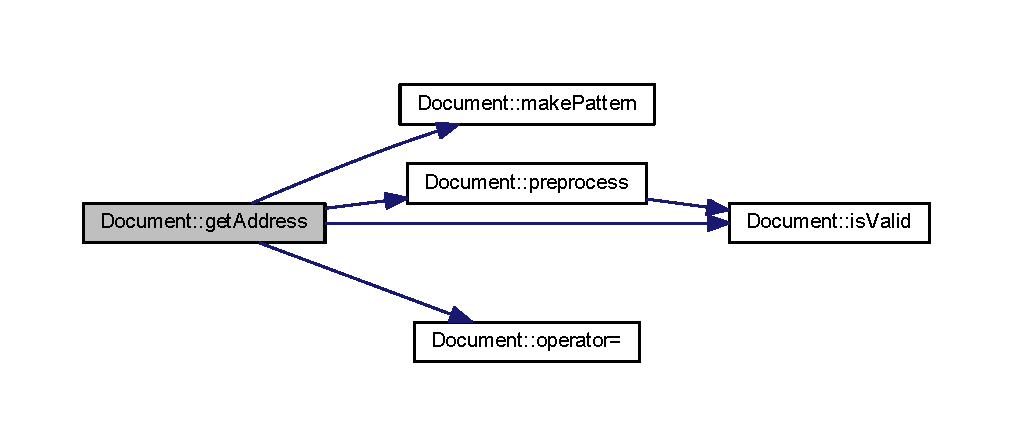
\includegraphics[width=350pt]{class_document_aba3c51ac1b4cb63dd9235aaa9e5ab6f0_cgraph}
\end{center}
\end{figure}


\index{Document@{Document}!is\+Valid@{is\+Valid}}
\index{is\+Valid@{is\+Valid}!Document@{Document}}
\subsubsection[{\texorpdfstring{is\+Valid(char c)}{isValid(char c)}}]{\setlength{\rightskip}{0pt plus 5cm}bool Document\+::is\+Valid (
\begin{DoxyParamCaption}
\item[{char}]{c}
\end{DoxyParamCaption}
)\hspace{0.3cm}{\ttfamily [protected]}}\hypertarget{class_document_ae81119fe62cb6c73bff4c9283c97884f}{}\label{class_document_ae81119fe62cb6c73bff4c9283c97884f}


Here is the caller graph for this function\+:\nopagebreak
\begin{figure}[H]
\begin{center}
\leavevmode
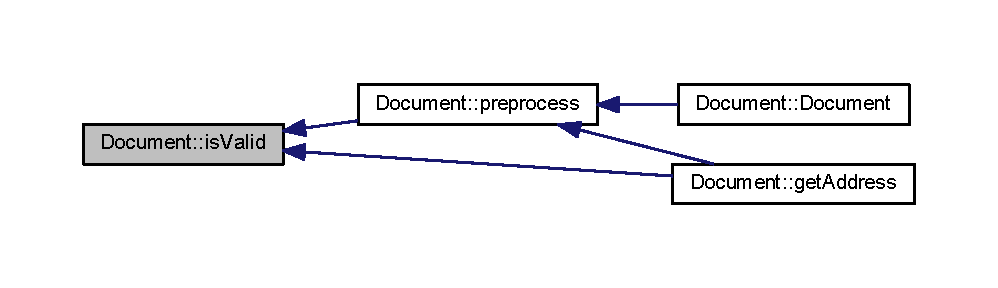
\includegraphics[width=350pt]{class_document_ae81119fe62cb6c73bff4c9283c97884f_icgraph}
\end{center}
\end{figure}


\index{Document@{Document}!K\+MP@{K\+MP}}
\index{K\+MP@{K\+MP}!Document@{Document}}
\subsubsection[{\texorpdfstring{K\+M\+P()}{KMP()}}]{\setlength{\rightskip}{0pt plus 5cm}void Document\+::\+K\+MP (
\begin{DoxyParamCaption}
{}
\end{DoxyParamCaption}
)}\hypertarget{class_document_aa02349519b475996d1206dfbbcaab349}{}\label{class_document_aa02349519b475996d1206dfbbcaab349}


Perdorm K\+MP algorithm for this document. 



Here is the call graph for this function\+:\nopagebreak
\begin{figure}[H]
\begin{center}
\leavevmode
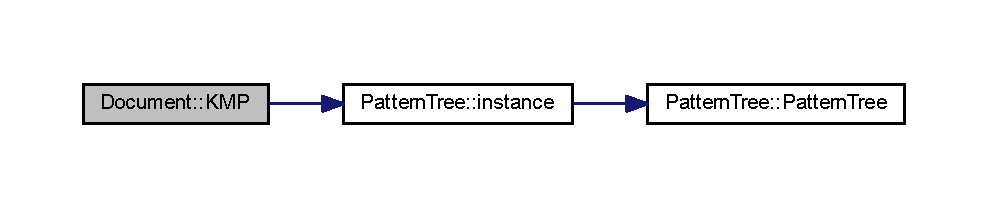
\includegraphics[width=350pt]{class_document_aa02349519b475996d1206dfbbcaab349_cgraph}
\end{center}
\end{figure}


\index{Document@{Document}!make\+Pattern@{make\+Pattern}}
\index{make\+Pattern@{make\+Pattern}!Document@{Document}}
\subsubsection[{\texorpdfstring{make\+Pattern()}{makePattern()}}]{\setlength{\rightskip}{0pt plus 5cm}void Document\+::make\+Pattern (
\begin{DoxyParamCaption}
{}
\end{DoxyParamCaption}
)\hspace{0.3cm}{\ttfamily [protected]}}\hypertarget{class_document_a019a44be44bd7b548ea32e4c699bed49}{}\label{class_document_a019a44be44bd7b548ea32e4c699bed49}


Make the patterns with winnowing algorithm. 



Here is the caller graph for this function\+:\nopagebreak
\begin{figure}[H]
\begin{center}
\leavevmode
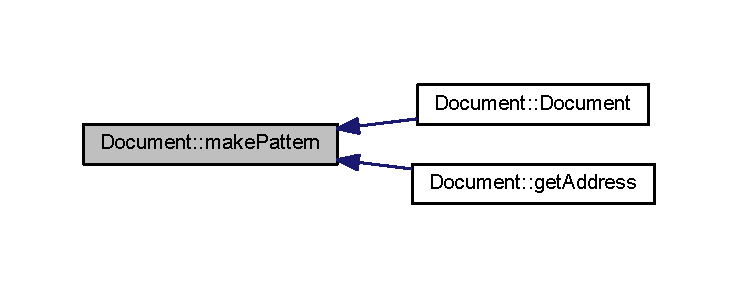
\includegraphics[width=350pt]{class_document_a019a44be44bd7b548ea32e4c699bed49_icgraph}
\end{center}
\end{figure}


\index{Document@{Document}!operator=@{operator=}}
\index{operator=@{operator=}!Document@{Document}}
\subsubsection[{\texorpdfstring{operator=(const Document \&other)}{operator=(const Document &other)}}]{\setlength{\rightskip}{0pt plus 5cm}{\bf Document}\& Document\+::operator= (
\begin{DoxyParamCaption}
\item[{const {\bf Document} \&}]{other}
\end{DoxyParamCaption}
)\hspace{0.3cm}{\ttfamily [private]}}\hypertarget{class_document_a4ccdb9185bd311793ad385564553153c}{}\label{class_document_a4ccdb9185bd311793ad385564553153c}


Here is the caller graph for this function\+:
\nopagebreak
\begin{figure}[H]
\begin{center}
\leavevmode
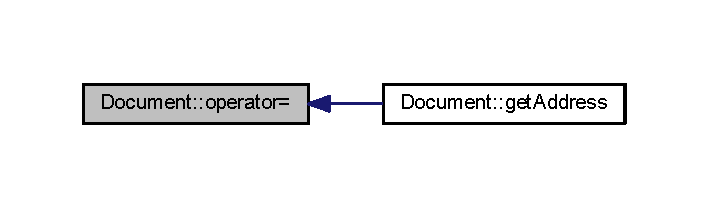
\includegraphics[width=340pt]{class_document_a4ccdb9185bd311793ad385564553153c_icgraph}
\end{center}
\end{figure}


\index{Document@{Document}!preprocess@{preprocess}}
\index{preprocess@{preprocess}!Document@{Document}}
\subsubsection[{\texorpdfstring{preprocess()}{preprocess()}}]{\setlength{\rightskip}{0pt plus 5cm}void Document\+::preprocess (
\begin{DoxyParamCaption}
{}
\end{DoxyParamCaption}
)\hspace{0.3cm}{\ttfamily [protected]}}\hypertarget{class_document_a508bc7255ec6ddf96d0d7078ff0d1229}{}\label{class_document_a508bc7255ec6ddf96d0d7078ff0d1229}
Remove spaces and taps and etc; Need to replace comments Need to add replacement 

Here is the call graph for this function\+:\nopagebreak
\begin{figure}[H]
\begin{center}
\leavevmode
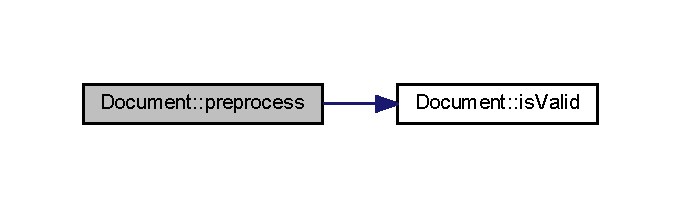
\includegraphics[width=327pt]{class_document_a508bc7255ec6ddf96d0d7078ff0d1229_cgraph}
\end{center}
\end{figure}




Here is the caller graph for this function\+:\nopagebreak
\begin{figure}[H]
\begin{center}
\leavevmode
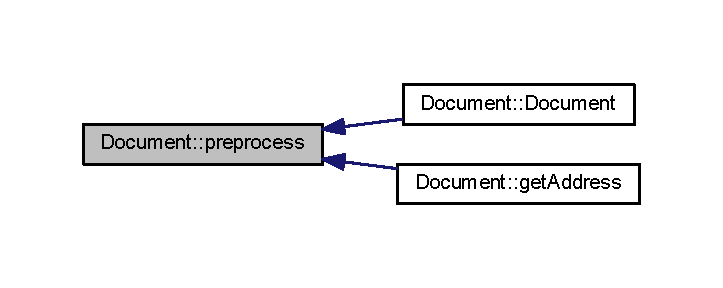
\includegraphics[width=347pt]{class_document_a508bc7255ec6ddf96d0d7078ff0d1229_icgraph}
\end{center}
\end{figure}


\index{Document@{Document}!Rabin\+Karp@{Rabin\+Karp}}
\index{Rabin\+Karp@{Rabin\+Karp}!Document@{Document}}
\subsubsection[{\texorpdfstring{Rabin\+Karp()}{RabinKarp()}}]{\setlength{\rightskip}{0pt plus 5cm}void Document\+::\+Rabin\+Karp (
\begin{DoxyParamCaption}
{}
\end{DoxyParamCaption}
)}\hypertarget{class_document_a607bc11ebda64c08fd22c8ca7aa373d3}{}\label{class_document_a607bc11ebda64c08fd22c8ca7aa373d3}


Perform Rabin-\/\+Karp algorithm for this document. 



Here is the call graph for this function\+:\nopagebreak
\begin{figure}[H]
\begin{center}
\leavevmode
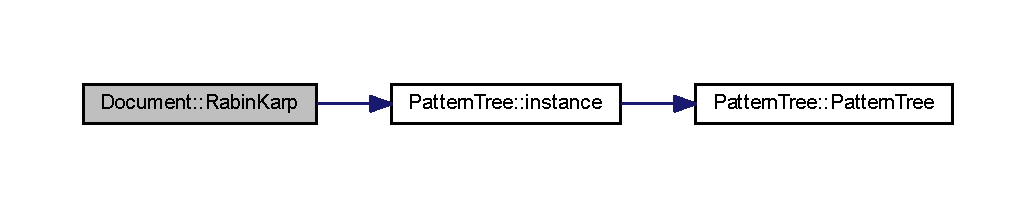
\includegraphics[width=350pt]{class_document_a607bc11ebda64c08fd22c8ca7aa373d3_cgraph}
\end{center}
\end{figure}




\subsection{Member Data Documentation}
\index{Document@{Document}!m\+\_\+address@{m\+\_\+address}}
\index{m\+\_\+address@{m\+\_\+address}!Document@{Document}}
\subsubsection[{\texorpdfstring{m\+\_\+address}{m_address}}]{\setlength{\rightskip}{0pt plus 5cm}std\+::string Document\+::m\+\_\+address\hspace{0.3cm}{\ttfamily [private]}}\hypertarget{class_document_a20ece3a3a1e633e381d28813ad76a088}{}\label{class_document_a20ece3a3a1e633e381d28813ad76a088}
\index{Document@{Document}!m\+\_\+content@{m\+\_\+content}}
\index{m\+\_\+content@{m\+\_\+content}!Document@{Document}}
\subsubsection[{\texorpdfstring{m\+\_\+content}{m_content}}]{\setlength{\rightskip}{0pt plus 5cm}std\+::string Document\+::m\+\_\+content\hspace{0.3cm}{\ttfamily [private]}}\hypertarget{class_document_a7d965b64a228ab63761ec4440a5549e0}{}\label{class_document_a7d965b64a228ab63761ec4440a5549e0}
\index{Document@{Document}!m\+\_\+patterns@{m\+\_\+patterns}}
\index{m\+\_\+patterns@{m\+\_\+patterns}!Document@{Document}}
\subsubsection[{\texorpdfstring{m\+\_\+patterns}{m_patterns}}]{\setlength{\rightskip}{0pt plus 5cm}std\+::vector$<${\bf Pattern}$>$ Document\+::m\+\_\+patterns\hspace{0.3cm}{\ttfamily [private]}}\hypertarget{class_document_a6cdddf9610a671723515bb6c71553870}{}\label{class_document_a6cdddf9610a671723515bb6c71553870}

\hypertarget{class_homework}{}\section{Homework Class Reference}
\label{class_homework}\index{Homework@{Homework}}
\subsection*{Public Types}
\begin{DoxyCompactItemize}
\item 
enum \hyperlink{class_homework_a6509dc051b3763d7fea21b4557d3e79e}{Homework\+Type} \{ \hyperlink{class_homework_a6509dc051b3763d7fea21b4557d3e79ea36e19dfd1e533060c7fe573d957186b7}{Single}, 
\hyperlink{class_homework_a6509dc051b3763d7fea21b4557d3e79ea70ece26b542060114ccdffac5e147ee9}{Multiple}
 \}
\end{DoxyCompactItemize}
\subsection*{Public Member Functions}
\begin{DoxyCompactItemize}
\item 
\hyperlink{class_homework_aff55dea2a7a6958a7c05c1e843061f81}{Homework} (std\+::string path, \hyperlink{class_homework_a6509dc051b3763d7fea21b4557d3e79e}{Homework\+Type} type)
\begin{DoxyCompactList}\small\item\em Initialization and build the whole file system. \end{DoxyCompactList}\end{DoxyCompactItemize}
\subsection*{Protected Member Functions}
\begin{DoxyCompactItemize}
\item 
bool \hyperlink{class_homework_aab839a8b3d15dbf849b018e2295aecc2}{find\+Single} (std\+::string file\+Path)
\item 
bool \hyperlink{class_homework_aef97adc1d880c7aaf5870d70b05777c0}{find\+Multiple} (std\+::string file\+Path)
\item 
void \hyperlink{class_homework_ae7c7babeff4d2f82b9ac0b139e92701e}{dfs\+Folder} (std\+::string folder\+Path, std\+::vector$<$ std\+::string $>$ \&address)
\end{DoxyCompactItemize}
\subsection*{Private Attributes}
\begin{DoxyCompactItemize}
\item 
\hyperlink{class_homework_a6509dc051b3763d7fea21b4557d3e79e}{Homework\+Type} \hyperlink{class_homework_a2a684368d7bdfaa95ee102e4fa6372ba}{m\+\_\+type}
\item 
std\+::string \hyperlink{class_homework_acfd58f754bd1712de9903dc986dc6d1e}{m\+\_\+path}
\item 
std\+::vector$<$ \hyperlink{class_project}{Project} $>$ \hyperlink{class_homework_a7d9479cfebf02074e2ac340561f7fb8e}{m\+\_\+projects}
\end{DoxyCompactItemize}


\subsection{Member Enumeration Documentation}
\index{Homework@{Homework}!Homework\+Type@{Homework\+Type}}
\index{Homework\+Type@{Homework\+Type}!Homework@{Homework}}
\subsubsection[{\texorpdfstring{Homework\+Type}{HomeworkType}}]{\setlength{\rightskip}{0pt plus 5cm}enum {\bf Homework\+::\+Homework\+Type}}\hypertarget{class_homework_a6509dc051b3763d7fea21b4557d3e79e}{}\label{class_homework_a6509dc051b3763d7fea21b4557d3e79e}
\begin{Desc}
\item[Enumerator]\par
\begin{description}
\index{Single@{Single}!Homework@{Homework}}\index{Homework@{Homework}!Single@{Single}}\item[{\em 
Single\hypertarget{class_homework_a6509dc051b3763d7fea21b4557d3e79ea36e19dfd1e533060c7fe573d957186b7}{}\label{class_homework_a6509dc051b3763d7fea21b4557d3e79ea36e19dfd1e533060c7fe573d957186b7}
}]\index{Multiple@{Multiple}!Homework@{Homework}}\index{Homework@{Homework}!Multiple@{Multiple}}\item[{\em 
Multiple\hypertarget{class_homework_a6509dc051b3763d7fea21b4557d3e79ea70ece26b542060114ccdffac5e147ee9}{}\label{class_homework_a6509dc051b3763d7fea21b4557d3e79ea70ece26b542060114ccdffac5e147ee9}
}]\end{description}
\end{Desc}


\subsection{Constructor \& Destructor Documentation}
\index{Homework@{Homework}!Homework@{Homework}}
\index{Homework@{Homework}!Homework@{Homework}}
\subsubsection[{\texorpdfstring{Homework(std\+::string path, Homework\+Type type)}{Homework(std::string path, HomeworkType type)}}]{\setlength{\rightskip}{0pt plus 5cm}Homework\+::\+Homework (
\begin{DoxyParamCaption}
\item[{std\+::string}]{path, }
\item[{{\bf Homework\+Type}}]{type}
\end{DoxyParamCaption}
)}\hypertarget{class_homework_aff55dea2a7a6958a7c05c1e843061f81}{}\label{class_homework_aff55dea2a7a6958a7c05c1e843061f81}


Initialization and build the whole file system. 



Here is the call graph for this function\+:\nopagebreak
\begin{figure}[H]
\begin{center}
\leavevmode
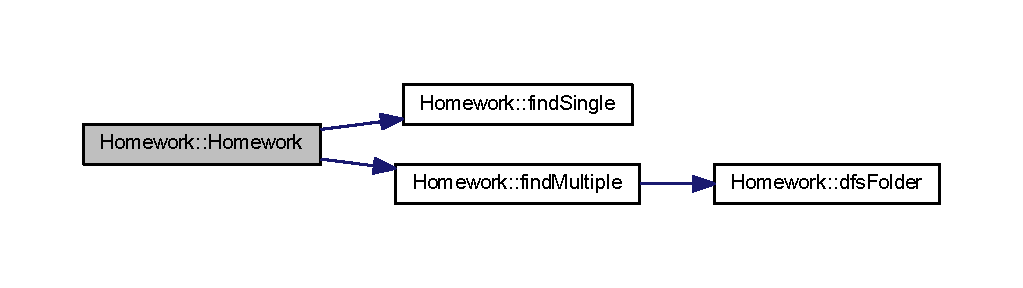
\includegraphics[width=350pt]{class_homework_aff55dea2a7a6958a7c05c1e843061f81_cgraph}
\end{center}
\end{figure}




\subsection{Member Function Documentation}
\index{Homework@{Homework}!dfs\+Folder@{dfs\+Folder}}
\index{dfs\+Folder@{dfs\+Folder}!Homework@{Homework}}
\subsubsection[{\texorpdfstring{dfs\+Folder(std\+::string folder\+Path, std\+::vector$<$ std\+::string $>$ \&address)}{dfsFolder(std::string folderPath, std::vector< std::string > &address)}}]{\setlength{\rightskip}{0pt plus 5cm}void Homework\+::dfs\+Folder (
\begin{DoxyParamCaption}
\item[{std\+::string}]{folder\+Path, }
\item[{std\+::vector$<$ std\+::string $>$ \&}]{address}
\end{DoxyParamCaption}
)\hspace{0.3cm}{\ttfamily [protected]}}\hypertarget{class_homework_ae7c7babeff4d2f82b9ac0b139e92701e}{}\label{class_homework_ae7c7babeff4d2f82b9ac0b139e92701e}


Here is the caller graph for this function\+:\nopagebreak
\begin{figure}[H]
\begin{center}
\leavevmode
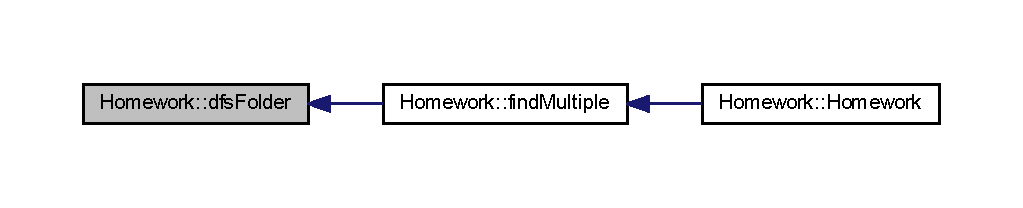
\includegraphics[width=350pt]{class_homework_ae7c7babeff4d2f82b9ac0b139e92701e_icgraph}
\end{center}
\end{figure}


\index{Homework@{Homework}!find\+Multiple@{find\+Multiple}}
\index{find\+Multiple@{find\+Multiple}!Homework@{Homework}}
\subsubsection[{\texorpdfstring{find\+Multiple(std\+::string file\+Path)}{findMultiple(std::string filePath)}}]{\setlength{\rightskip}{0pt plus 5cm}bool Homework\+::find\+Multiple (
\begin{DoxyParamCaption}
\item[{std\+::string}]{file\+Path}
\end{DoxyParamCaption}
)\hspace{0.3cm}{\ttfamily [protected]}}\hypertarget{class_homework_aef97adc1d880c7aaf5870d70b05777c0}{}\label{class_homework_aef97adc1d880c7aaf5870d70b05777c0}


Here is the call graph for this function\+:\nopagebreak
\begin{figure}[H]
\begin{center}
\leavevmode
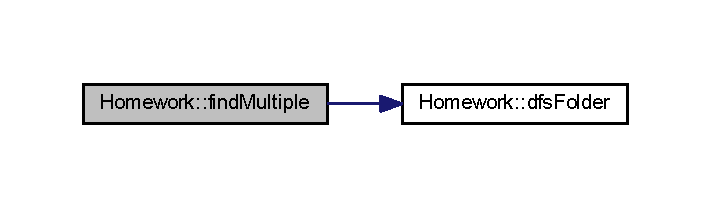
\includegraphics[width=341pt]{class_homework_aef97adc1d880c7aaf5870d70b05777c0_cgraph}
\end{center}
\end{figure}




Here is the caller graph for this function\+:\nopagebreak
\begin{figure}[H]
\begin{center}
\leavevmode
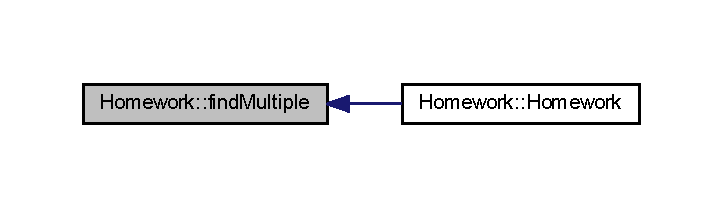
\includegraphics[width=347pt]{class_homework_aef97adc1d880c7aaf5870d70b05777c0_icgraph}
\end{center}
\end{figure}


\index{Homework@{Homework}!find\+Single@{find\+Single}}
\index{find\+Single@{find\+Single}!Homework@{Homework}}
\subsubsection[{\texorpdfstring{find\+Single(std\+::string file\+Path)}{findSingle(std::string filePath)}}]{\setlength{\rightskip}{0pt plus 5cm}bool Homework\+::find\+Single (
\begin{DoxyParamCaption}
\item[{std\+::string}]{file\+Path}
\end{DoxyParamCaption}
)\hspace{0.3cm}{\ttfamily [protected]}}\hypertarget{class_homework_aab839a8b3d15dbf849b018e2295aecc2}{}\label{class_homework_aab839a8b3d15dbf849b018e2295aecc2}


Here is the caller graph for this function\+:\nopagebreak
\begin{figure}[H]
\begin{center}
\leavevmode
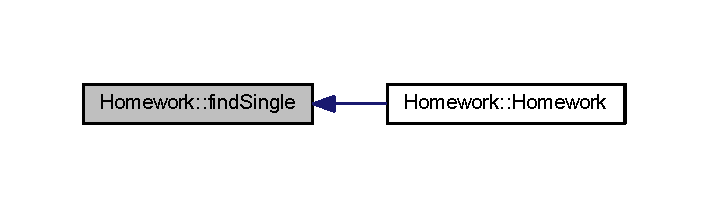
\includegraphics[width=340pt]{class_homework_aab839a8b3d15dbf849b018e2295aecc2_icgraph}
\end{center}
\end{figure}




\subsection{Member Data Documentation}
\index{Homework@{Homework}!m\+\_\+path@{m\+\_\+path}}
\index{m\+\_\+path@{m\+\_\+path}!Homework@{Homework}}
\subsubsection[{\texorpdfstring{m\+\_\+path}{m_path}}]{\setlength{\rightskip}{0pt plus 5cm}std\+::string Homework\+::m\+\_\+path\hspace{0.3cm}{\ttfamily [private]}}\hypertarget{class_homework_acfd58f754bd1712de9903dc986dc6d1e}{}\label{class_homework_acfd58f754bd1712de9903dc986dc6d1e}
\index{Homework@{Homework}!m\+\_\+projects@{m\+\_\+projects}}
\index{m\+\_\+projects@{m\+\_\+projects}!Homework@{Homework}}
\subsubsection[{\texorpdfstring{m\+\_\+projects}{m_projects}}]{\setlength{\rightskip}{0pt plus 5cm}std\+::vector$<${\bf Project}$>$ Homework\+::m\+\_\+projects\hspace{0.3cm}{\ttfamily [private]}}\hypertarget{class_homework_a7d9479cfebf02074e2ac340561f7fb8e}{}\label{class_homework_a7d9479cfebf02074e2ac340561f7fb8e}
\index{Homework@{Homework}!m\+\_\+type@{m\+\_\+type}}
\index{m\+\_\+type@{m\+\_\+type}!Homework@{Homework}}
\subsubsection[{\texorpdfstring{m\+\_\+type}{m_type}}]{\setlength{\rightskip}{0pt plus 5cm}{\bf Homework\+Type} Homework\+::m\+\_\+type\hspace{0.3cm}{\ttfamily [private]}}\hypertarget{class_homework_a2a684368d7bdfaa95ee102e4fa6372ba}{}\label{class_homework_a2a684368d7bdfaa95ee102e4fa6372ba}

\hypertarget{class_pattern}{}\section{Pattern Class Reference}
\label{class_pattern}\index{Pattern@{Pattern}}


Storing patterns from a document.  




Collaboration diagram for Pattern\+:
\nopagebreak
\begin{figure}[H]
\begin{center}
\leavevmode
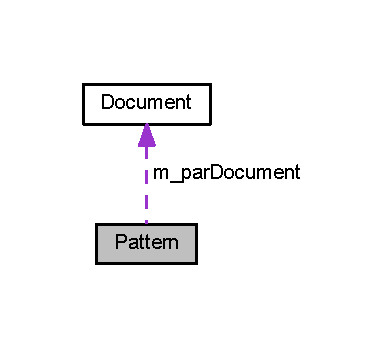
\includegraphics[width=186pt]{class_pattern__coll__graph}
\end{center}
\end{figure}
\subsection*{Public Member Functions}
\begin{DoxyCompactItemize}
\item 
\hyperlink{class_pattern_ada73ecc1fc5e4d94f30a8161feef67cf}{Pattern} (\hyperlink{class_document}{Document} \&par\+Document, std\+::string pattern, int pos)
\begin{DoxyCompactList}\small\item\em The only constructor. \end{DoxyCompactList}\item 
bool \hyperlink{class_pattern_a157a34771b4c550a7cf528f09fa685b5}{operator$<$} (const \hyperlink{class_pattern}{Pattern} \&right)
\begin{DoxyCompactList}\small\item\em operator $<$ for inserting into \hyperlink{class_pattern_tree}{Pattern\+Tree} \end{DoxyCompactList}\item 
long long int \hyperlink{class_pattern_ab6c1a23c63162c8e9bc27061e9370ed1}{get\+Hash} () const 
\item 
int \hyperlink{class_pattern_a371d9dad975d97190b969ee6e77178c0}{get\+Length} () const 
\item 
\hyperlink{class_document}{Document} $\ast$ \hyperlink{class_pattern_aba85629c60347a4f3c81bd7088af4c55}{get\+Par\+Document} ()
\item 
std\+::string \hyperlink{class_pattern_ad4f3ad6d391eea8c6fd95efdf7f7246d}{get\+Pattern} () const 
\item 
void \hyperlink{class_pattern_a44a70e6aff49a25fa068487e3d9f0fa3}{print} () const 
\begin{DoxyCompactList}\small\item\em print basic information about the pattern \end{DoxyCompactList}\end{DoxyCompactItemize}
\subsection*{Protected Member Functions}
\begin{DoxyCompactItemize}
\item 
void \hyperlink{class_pattern_a8c7f0e27f620c00de00d097c84e9d6c3}{calc\+Hash} ()
\end{DoxyCompactItemize}
\subsection*{Private Member Functions}
\begin{DoxyCompactItemize}
\item 
\hyperlink{class_pattern}{Pattern} \& \hyperlink{class_pattern_a69f59394d218d0e476ef9259130e6bef}{operator=} (const \hyperlink{class_pattern}{Pattern} \&other)
\end{DoxyCompactItemize}
\subsection*{Private Attributes}
\begin{DoxyCompactItemize}
\item 
std\+::string \hyperlink{class_pattern_a492ef4124f2dfebee1babe983cf3f726}{m\+\_\+pattern}
\item 
int \hyperlink{class_pattern_aa5b42830eafc550988e9156e4c370f67}{m\+\_\+pos}
\item 
long long int \hyperlink{class_pattern_ad2d90cf1c416dd89f29e7da860a02bfb}{m\+\_\+hash}
\item 
\hyperlink{class_document}{Document} $\ast$ \hyperlink{class_pattern_a3ce8a1a5ba37412027278315935c06b8}{m\+\_\+par\+Document}
\end{DoxyCompactItemize}


\subsection{Detailed Description}
Storing patterns from a document. 

\subsection{Constructor \& Destructor Documentation}
\index{Pattern@{Pattern}!Pattern@{Pattern}}
\index{Pattern@{Pattern}!Pattern@{Pattern}}
\subsubsection[{\texorpdfstring{Pattern(\+Document \&par\+Document, std\+::string pattern, int pos)}{Pattern(Document &parDocument, std::string pattern, int pos)}}]{\setlength{\rightskip}{0pt plus 5cm}Pattern\+::\+Pattern (
\begin{DoxyParamCaption}
\item[{{\bf Document} \&}]{par\+Document, }
\item[{std\+::string}]{pattern, }
\item[{int}]{pos}
\end{DoxyParamCaption}
)}\hypertarget{class_pattern_ada73ecc1fc5e4d94f30a8161feef67cf}{}\label{class_pattern_ada73ecc1fc5e4d94f30a8161feef67cf}


The only constructor. 



Here is the call graph for this function\+:\nopagebreak
\begin{figure}[H]
\begin{center}
\leavevmode
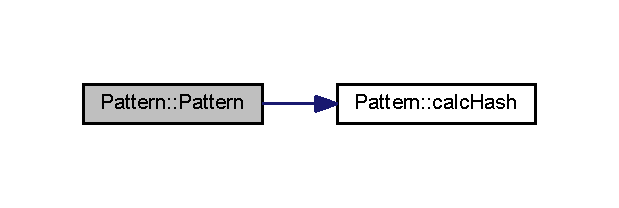
\includegraphics[width=297pt]{class_pattern_ada73ecc1fc5e4d94f30a8161feef67cf_cgraph}
\end{center}
\end{figure}




\subsection{Member Function Documentation}
\index{Pattern@{Pattern}!calc\+Hash@{calc\+Hash}}
\index{calc\+Hash@{calc\+Hash}!Pattern@{Pattern}}
\subsubsection[{\texorpdfstring{calc\+Hash()}{calcHash()}}]{\setlength{\rightskip}{0pt plus 5cm}void Pattern\+::calc\+Hash (
\begin{DoxyParamCaption}
{}
\end{DoxyParamCaption}
)\hspace{0.3cm}{\ttfamily [protected]}}\hypertarget{class_pattern_a8c7f0e27f620c00de00d097c84e9d6c3}{}\label{class_pattern_a8c7f0e27f620c00de00d097c84e9d6c3}


Here is the caller graph for this function\+:\nopagebreak
\begin{figure}[H]
\begin{center}
\leavevmode
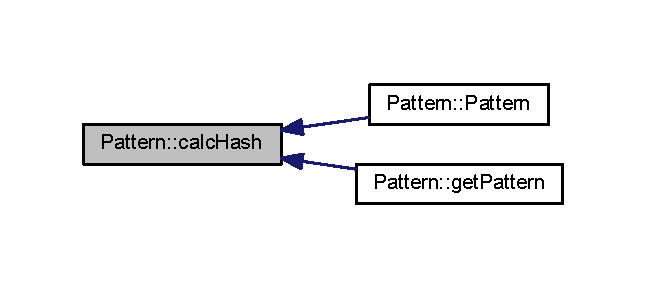
\includegraphics[width=310pt]{class_pattern_a8c7f0e27f620c00de00d097c84e9d6c3_icgraph}
\end{center}
\end{figure}


\index{Pattern@{Pattern}!get\+Hash@{get\+Hash}}
\index{get\+Hash@{get\+Hash}!Pattern@{Pattern}}
\subsubsection[{\texorpdfstring{get\+Hash() const }{getHash() const }}]{\setlength{\rightskip}{0pt plus 5cm}long long int Pattern\+::get\+Hash (
\begin{DoxyParamCaption}
{}
\end{DoxyParamCaption}
) const\hspace{0.3cm}{\ttfamily [inline]}}\hypertarget{class_pattern_ab6c1a23c63162c8e9bc27061e9370ed1}{}\label{class_pattern_ab6c1a23c63162c8e9bc27061e9370ed1}
\begin{DoxyReturn}{Returns}
The hash value. 
\end{DoxyReturn}


Here is the caller graph for this function\+:\nopagebreak
\begin{figure}[H]
\begin{center}
\leavevmode
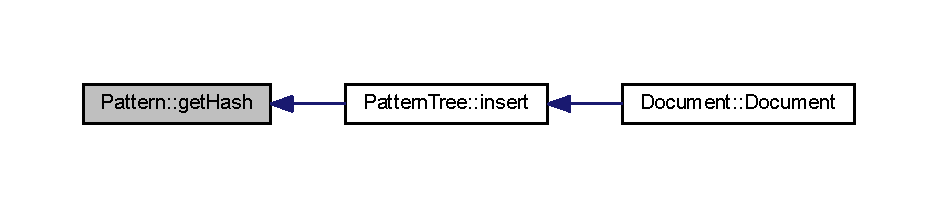
\includegraphics[width=350pt]{class_pattern_ab6c1a23c63162c8e9bc27061e9370ed1_icgraph}
\end{center}
\end{figure}


\index{Pattern@{Pattern}!get\+Length@{get\+Length}}
\index{get\+Length@{get\+Length}!Pattern@{Pattern}}
\subsubsection[{\texorpdfstring{get\+Length() const }{getLength() const }}]{\setlength{\rightskip}{0pt plus 5cm}int Pattern\+::get\+Length (
\begin{DoxyParamCaption}
{}
\end{DoxyParamCaption}
) const\hspace{0.3cm}{\ttfamily [inline]}}\hypertarget{class_pattern_a371d9dad975d97190b969ee6e77178c0}{}\label{class_pattern_a371d9dad975d97190b969ee6e77178c0}
\begin{DoxyReturn}{Returns}
the length of the pattern. 
\end{DoxyReturn}
\index{Pattern@{Pattern}!get\+Par\+Document@{get\+Par\+Document}}
\index{get\+Par\+Document@{get\+Par\+Document}!Pattern@{Pattern}}
\subsubsection[{\texorpdfstring{get\+Par\+Document()}{getParDocument()}}]{\setlength{\rightskip}{0pt plus 5cm}{\bf Document}$\ast$ Pattern\+::get\+Par\+Document (
\begin{DoxyParamCaption}
{}
\end{DoxyParamCaption}
)\hspace{0.3cm}{\ttfamily [inline]}}\hypertarget{class_pattern_aba85629c60347a4f3c81bd7088af4c55}{}\label{class_pattern_aba85629c60347a4f3c81bd7088af4c55}
\begin{DoxyReturn}{Returns}
the address of the parent document. Note\+: need to use const here 
\end{DoxyReturn}
\index{Pattern@{Pattern}!get\+Pattern@{get\+Pattern}}
\index{get\+Pattern@{get\+Pattern}!Pattern@{Pattern}}
\subsubsection[{\texorpdfstring{get\+Pattern() const }{getPattern() const }}]{\setlength{\rightskip}{0pt plus 5cm}std\+::string Pattern\+::get\+Pattern (
\begin{DoxyParamCaption}
{}
\end{DoxyParamCaption}
) const\hspace{0.3cm}{\ttfamily [inline]}}\hypertarget{class_pattern_ad4f3ad6d391eea8c6fd95efdf7f7246d}{}\label{class_pattern_ad4f3ad6d391eea8c6fd95efdf7f7246d}


Here is the call graph for this function\+:
\nopagebreak
\begin{figure}[H]
\begin{center}
\leavevmode
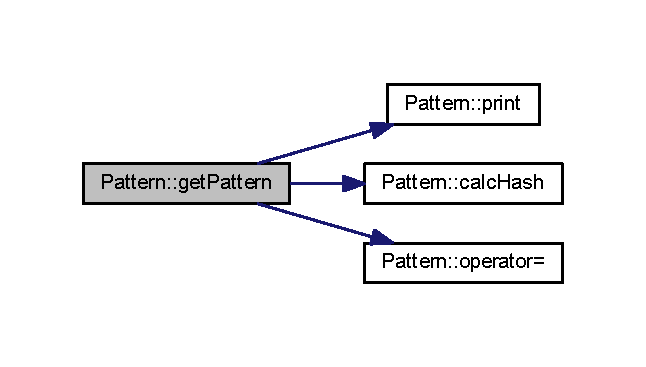
\includegraphics[width=310pt]{class_pattern_ad4f3ad6d391eea8c6fd95efdf7f7246d_cgraph}
\end{center}
\end{figure}


\index{Pattern@{Pattern}!operator$<$@{operator$<$}}
\index{operator$<$@{operator$<$}!Pattern@{Pattern}}
\subsubsection[{\texorpdfstring{operator$<$(const Pattern \&right)}{operator<(const Pattern &right)}}]{\setlength{\rightskip}{0pt plus 5cm}bool Pattern\+::operator$<$ (
\begin{DoxyParamCaption}
\item[{const {\bf Pattern} \&}]{right}
\end{DoxyParamCaption}
)\hspace{0.3cm}{\ttfamily [inline]}}\hypertarget{class_pattern_a157a34771b4c550a7cf528f09fa685b5}{}\label{class_pattern_a157a34771b4c550a7cf528f09fa685b5}


operator $<$ for inserting into \hyperlink{class_pattern_tree}{Pattern\+Tree} 

\index{Pattern@{Pattern}!operator=@{operator=}}
\index{operator=@{operator=}!Pattern@{Pattern}}
\subsubsection[{\texorpdfstring{operator=(const Pattern \&other)}{operator=(const Pattern &other)}}]{\setlength{\rightskip}{0pt plus 5cm}{\bf Pattern}\& Pattern\+::operator= (
\begin{DoxyParamCaption}
\item[{const {\bf Pattern} \&}]{other}
\end{DoxyParamCaption}
)\hspace{0.3cm}{\ttfamily [private]}}\hypertarget{class_pattern_a69f59394d218d0e476ef9259130e6bef}{}\label{class_pattern_a69f59394d218d0e476ef9259130e6bef}


Here is the caller graph for this function\+:
\nopagebreak
\begin{figure}[H]
\begin{center}
\leavevmode
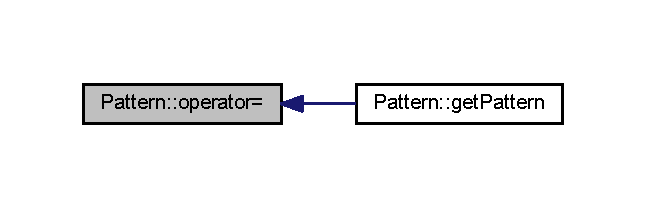
\includegraphics[width=310pt]{class_pattern_a69f59394d218d0e476ef9259130e6bef_icgraph}
\end{center}
\end{figure}


\index{Pattern@{Pattern}!print@{print}}
\index{print@{print}!Pattern@{Pattern}}
\subsubsection[{\texorpdfstring{print() const }{print() const }}]{\setlength{\rightskip}{0pt plus 5cm}void Pattern\+::print (
\begin{DoxyParamCaption}
{}
\end{DoxyParamCaption}
) const}\hypertarget{class_pattern_a44a70e6aff49a25fa068487e3d9f0fa3}{}\label{class_pattern_a44a70e6aff49a25fa068487e3d9f0fa3}


print basic information about the pattern 



Here is the caller graph for this function\+:\nopagebreak
\begin{figure}[H]
\begin{center}
\leavevmode
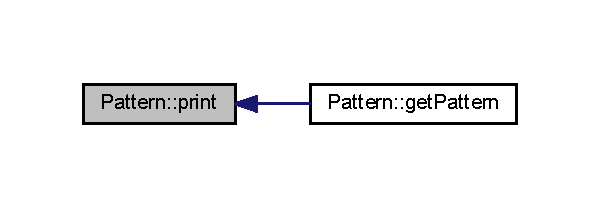
\includegraphics[width=288pt]{class_pattern_a44a70e6aff49a25fa068487e3d9f0fa3_icgraph}
\end{center}
\end{figure}




\subsection{Member Data Documentation}
\index{Pattern@{Pattern}!m\+\_\+hash@{m\+\_\+hash}}
\index{m\+\_\+hash@{m\+\_\+hash}!Pattern@{Pattern}}
\subsubsection[{\texorpdfstring{m\+\_\+hash}{m_hash}}]{\setlength{\rightskip}{0pt plus 5cm}long long int Pattern\+::m\+\_\+hash\hspace{0.3cm}{\ttfamily [private]}}\hypertarget{class_pattern_ad2d90cf1c416dd89f29e7da860a02bfb}{}\label{class_pattern_ad2d90cf1c416dd89f29e7da860a02bfb}
\index{Pattern@{Pattern}!m\+\_\+par\+Document@{m\+\_\+par\+Document}}
\index{m\+\_\+par\+Document@{m\+\_\+par\+Document}!Pattern@{Pattern}}
\subsubsection[{\texorpdfstring{m\+\_\+par\+Document}{m_parDocument}}]{\setlength{\rightskip}{0pt plus 5cm}{\bf Document}$\ast$ Pattern\+::m\+\_\+par\+Document\hspace{0.3cm}{\ttfamily [private]}}\hypertarget{class_pattern_a3ce8a1a5ba37412027278315935c06b8}{}\label{class_pattern_a3ce8a1a5ba37412027278315935c06b8}
\index{Pattern@{Pattern}!m\+\_\+pattern@{m\+\_\+pattern}}
\index{m\+\_\+pattern@{m\+\_\+pattern}!Pattern@{Pattern}}
\subsubsection[{\texorpdfstring{m\+\_\+pattern}{m_pattern}}]{\setlength{\rightskip}{0pt plus 5cm}std\+::string Pattern\+::m\+\_\+pattern\hspace{0.3cm}{\ttfamily [private]}}\hypertarget{class_pattern_a492ef4124f2dfebee1babe983cf3f726}{}\label{class_pattern_a492ef4124f2dfebee1babe983cf3f726}
\index{Pattern@{Pattern}!m\+\_\+pos@{m\+\_\+pos}}
\index{m\+\_\+pos@{m\+\_\+pos}!Pattern@{Pattern}}
\subsubsection[{\texorpdfstring{m\+\_\+pos}{m_pos}}]{\setlength{\rightskip}{0pt plus 5cm}int Pattern\+::m\+\_\+pos\hspace{0.3cm}{\ttfamily [private]}}\hypertarget{class_pattern_aa5b42830eafc550988e9156e4c370f67}{}\label{class_pattern_aa5b42830eafc550988e9156e4c370f67}

\hypertarget{class_pattern_tree}{}\section{PatternTree Class Reference}
\label{class_pattern_tree}\index{PatternTree@{PatternTree}}


Collaboration diagram for PatternTree:
\nopagebreak
\begin{figure}[H]
\begin{center}
\leavevmode
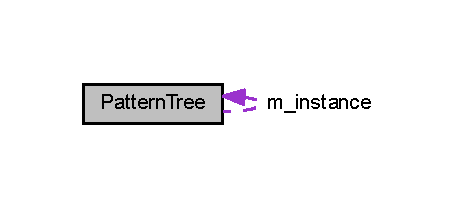
\includegraphics[width=219pt]{class_pattern_tree__coll__graph}
\end{center}
\end{figure}
\subsection*{Public Member Functions}
\begin{DoxyCompactItemize}
\item 
\hyperlink{class_pattern_tree_a8c393d9dc7966220803f670062d81cb5}{PatternTree} ()
\item 
void \hyperlink{class_pattern_tree_aeedfa28c34ce69dc494675e9662bd60b}{destroy} ()
\item 
void \hyperlink{class_pattern_tree_af698c6d454803b5debff21fe19eecab5}{insert} (const \hyperlink{class_pattern}{Pattern} \&pattern)
\begin{DoxyCompactList}\small\item\em insert a pattern into the tree \end{DoxyCompactList}\item 
std::vector$<$ \hyperlink{class_pattern}{Pattern} $>$ \hyperlink{class_pattern_tree_a86ae88dfb3fd379e2b914590b5a2f896}{find} (const long long int hash)
\item 
std::vector$<$ \hyperlink{class_pattern}{Pattern} $>$ \hyperlink{class_pattern_tree_a01a7afad6ad98b8d5958096c54c45b1f}{getAll} ()
\item 
void \hyperlink{class_pattern_tree_a4db45bd0a698e9999c743f5ac05c33a6}{print} ()
\begin{DoxyCompactList}\small\item\em print some basic information about the tree \end{DoxyCompactList}\end{DoxyCompactItemize}
\subsection*{Static Public Member Functions}
\begin{DoxyCompactItemize}
\item 
static \hyperlink{class_pattern_tree}{PatternTree} $\ast$ \hyperlink{class_pattern_tree_ae3cb1d962789f1bfe37994eec207d493}{instance} ()
\end{DoxyCompactItemize}
\subsection*{Private Member Functions}
\begin{DoxyCompactItemize}
\item 
\hyperlink{class_pattern_tree_af84e0bf107c0fda11f1c971bfe3d9c4f}{PatternTree} (const \hyperlink{class_pattern_tree}{PatternTree} \&other)
\item 
\hyperlink{class_pattern_tree}{PatternTree} \& \hyperlink{class_pattern_tree_ad1ece378133ff4abb282cea9204b0ccc}{operator=} (const \hyperlink{class_pattern_tree}{PatternTree} \&right)
\end{DoxyCompactItemize}
\subsection*{Private Attributes}
\begin{DoxyCompactItemize}
\item 
patternMmap \hyperlink{class_pattern_tree_a8aa612fc369e9106116ad8e3e5b02021}{m\_tree}
\end{DoxyCompactItemize}
\subsection*{Static Private Attributes}
\begin{DoxyCompactItemize}
\item 
static \hyperlink{class_pattern_tree}{PatternTree} $\ast$ \hyperlink{class_pattern_tree_a84a86ffd132359390369421d1fb4c594}{m\_instance} = NULL
\end{DoxyCompactItemize}


\subsection{Detailed Description}
A tree with all patterns stored in it Singleton 

\subsection{Constructor \& Destructor Documentation}
\index{PatternTree@{PatternTree}!PatternTree@{PatternTree}}
\index{PatternTree@{PatternTree}!PatternTree@{PatternTree}}
\subsubsection[{\texorpdfstring{PatternTree()}{PatternTree()}}]{\setlength{\rightskip}{0pt plus 5cm}PatternTree::PatternTree (
\begin{DoxyParamCaption}
{}
\end{DoxyParamCaption}
)}\hypertarget{class_pattern_tree_a8c393d9dc7966220803f670062d81cb5}{}\label{class_pattern_tree_a8c393d9dc7966220803f670062d81cb5}


Here is the caller graph for this function:
\nopagebreak
\begin{figure}[H]
\begin{center}
\leavevmode
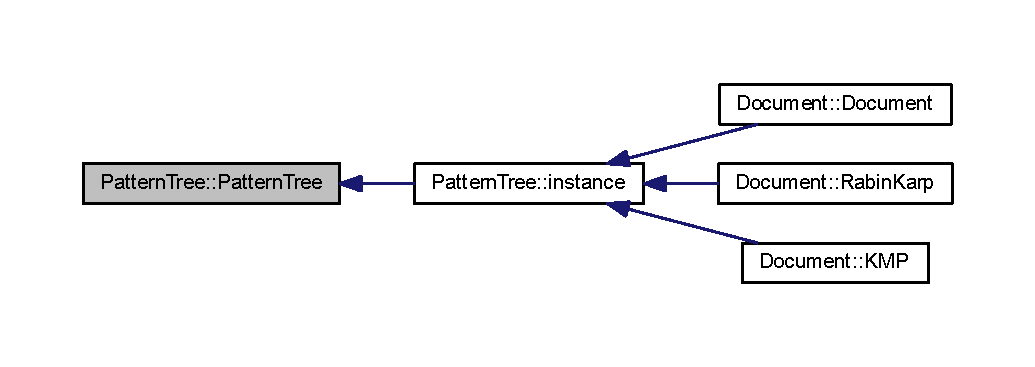
\includegraphics[width=350pt]{class_pattern_tree_a8c393d9dc7966220803f670062d81cb5_icgraph}
\end{center}
\end{figure}


\index{PatternTree@{PatternTree}!PatternTree@{PatternTree}}
\index{PatternTree@{PatternTree}!PatternTree@{PatternTree}}
\subsubsection[{\texorpdfstring{PatternTree(const PatternTree \&other)}{PatternTree(const PatternTree &other)}}]{\setlength{\rightskip}{0pt plus 5cm}PatternTree::PatternTree (
\begin{DoxyParamCaption}
\item[{const {\bf PatternTree} \&}]{other}
\end{DoxyParamCaption}
)\hspace{0.3cm}{\ttfamily [private]}}\hypertarget{class_pattern_tree_af84e0bf107c0fda11f1c971bfe3d9c4f}{}\label{class_pattern_tree_af84e0bf107c0fda11f1c971bfe3d9c4f}


\subsection{Member Function Documentation}
\index{PatternTree@{PatternTree}!destroy@{destroy}}
\index{destroy@{destroy}!PatternTree@{PatternTree}}
\subsubsection[{\texorpdfstring{destroy()}{destroy()}}]{\setlength{\rightskip}{0pt plus 5cm}void PatternTree::destroy (
\begin{DoxyParamCaption}
{}
\end{DoxyParamCaption}
)}\hypertarget{class_pattern_tree_aeedfa28c34ce69dc494675e9662bd60b}{}\label{class_pattern_tree_aeedfa28c34ce69dc494675e9662bd60b}
\index{PatternTree@{PatternTree}!find@{find}}
\index{find@{find}!PatternTree@{PatternTree}}
\subsubsection[{\texorpdfstring{find(const long long int hash)}{find(const long long int hash)}}]{\setlength{\rightskip}{0pt plus 5cm}std::vector$<$ {\bf Pattern} $>$ PatternTree::find (
\begin{DoxyParamCaption}
\item[{const long long int}]{hash}
\end{DoxyParamCaption}
)}\hypertarget{class_pattern_tree_a86ae88dfb3fd379e2b914590b5a2f896}{}\label{class_pattern_tree_a86ae88dfb3fd379e2b914590b5a2f896}
find a set of patterns with the same hash value in the tree Note: I cannot make it const... \index{PatternTree@{PatternTree}!getAll@{getAll}}
\index{getAll@{getAll}!PatternTree@{PatternTree}}
\subsubsection[{\texorpdfstring{getAll()}{getAll()}}]{\setlength{\rightskip}{0pt plus 5cm}std::vector$<$ {\bf Pattern} $>$ PatternTree::getAll (
\begin{DoxyParamCaption}
{}
\end{DoxyParamCaption}
)}\hypertarget{class_pattern_tree_a01a7afad6ad98b8d5958096c54c45b1f}{}\label{class_pattern_tree_a01a7afad6ad98b8d5958096c54c45b1f}
\index{PatternTree@{PatternTree}!insert@{insert}}
\index{insert@{insert}!PatternTree@{PatternTree}}
\subsubsection[{\texorpdfstring{insert(const Pattern \&pattern)}{insert(const Pattern &pattern)}}]{\setlength{\rightskip}{0pt plus 5cm}void PatternTree::insert (
\begin{DoxyParamCaption}
\item[{const {\bf Pattern} \&}]{pattern}
\end{DoxyParamCaption}
)}\hypertarget{class_pattern_tree_af698c6d454803b5debff21fe19eecab5}{}\label{class_pattern_tree_af698c6d454803b5debff21fe19eecab5}


insert a pattern into the tree 



Here is the call graph for this function:\nopagebreak
\begin{figure}[H]
\begin{center}
\leavevmode
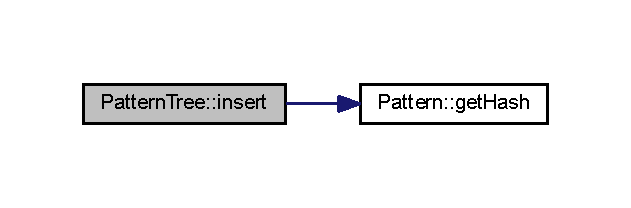
\includegraphics[width=303pt]{class_pattern_tree_af698c6d454803b5debff21fe19eecab5_cgraph}
\end{center}
\end{figure}




Here is the caller graph for this function:\nopagebreak
\begin{figure}[H]
\begin{center}
\leavevmode
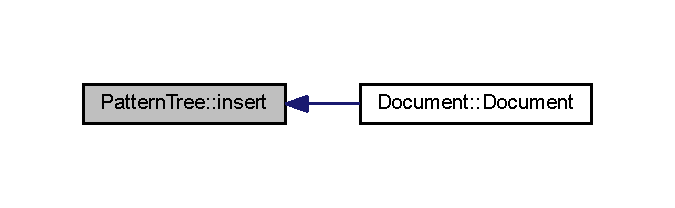
\includegraphics[width=324pt]{class_pattern_tree_af698c6d454803b5debff21fe19eecab5_icgraph}
\end{center}
\end{figure}


\index{PatternTree@{PatternTree}!instance@{instance}}
\index{instance@{instance}!PatternTree@{PatternTree}}
\subsubsection[{\texorpdfstring{instance()}{instance()}}]{\setlength{\rightskip}{0pt plus 5cm}{\bf PatternTree} $\ast$ PatternTree::instance (
\begin{DoxyParamCaption}
{}
\end{DoxyParamCaption}
)\hspace{0.3cm}{\ttfamily [static]}}\hypertarget{class_pattern_tree_ae3cb1d962789f1bfe37994eec207d493}{}\label{class_pattern_tree_ae3cb1d962789f1bfe37994eec207d493}


Here is the call graph for this function:\nopagebreak
\begin{figure}[H]
\begin{center}
\leavevmode
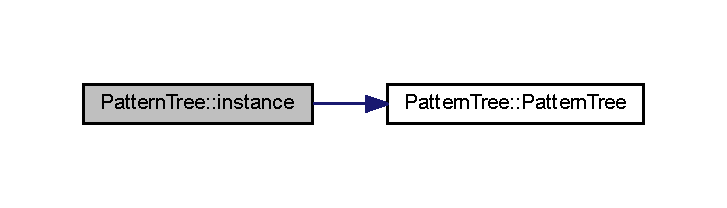
\includegraphics[width=349pt]{class_pattern_tree_ae3cb1d962789f1bfe37994eec207d493_cgraph}
\end{center}
\end{figure}




Here is the caller graph for this function:
\nopagebreak
\begin{figure}[H]
\begin{center}
\leavevmode
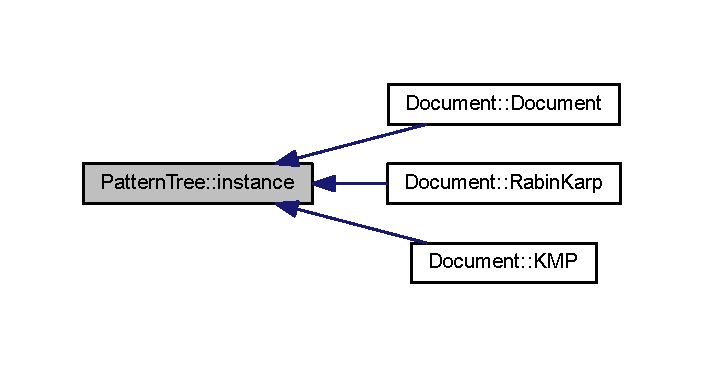
\includegraphics[width=338pt]{class_pattern_tree_ae3cb1d962789f1bfe37994eec207d493_icgraph}
\end{center}
\end{figure}


\index{PatternTree@{PatternTree}!operator=@{operator=}}
\index{operator=@{operator=}!PatternTree@{PatternTree}}
\subsubsection[{\texorpdfstring{operator=(const PatternTree \&right)}{operator=(const PatternTree &right)}}]{\setlength{\rightskip}{0pt plus 5cm}{\bf PatternTree}\& PatternTree::operator= (
\begin{DoxyParamCaption}
\item[{const {\bf PatternTree} \&}]{right}
\end{DoxyParamCaption}
)\hspace{0.3cm}{\ttfamily [private]}}\hypertarget{class_pattern_tree_ad1ece378133ff4abb282cea9204b0ccc}{}\label{class_pattern_tree_ad1ece378133ff4abb282cea9204b0ccc}
\index{PatternTree@{PatternTree}!print@{print}}
\index{print@{print}!PatternTree@{PatternTree}}
\subsubsection[{\texorpdfstring{print()}{print()}}]{\setlength{\rightskip}{0pt plus 5cm}void PatternTree::print (
\begin{DoxyParamCaption}
{}
\end{DoxyParamCaption}
)}\hypertarget{class_pattern_tree_a4db45bd0a698e9999c743f5ac05c33a6}{}\label{class_pattern_tree_a4db45bd0a698e9999c743f5ac05c33a6}


print some basic information about the tree 



Here is the caller graph for this function:\nopagebreak
\begin{figure}[H]
\begin{center}
\leavevmode
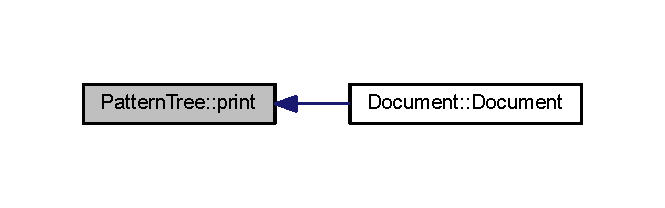
\includegraphics[width=319pt]{class_pattern_tree_a4db45bd0a698e9999c743f5ac05c33a6_icgraph}
\end{center}
\end{figure}




\subsection{Member Data Documentation}
\index{PatternTree@{PatternTree}!m\_instance@{m\_instance}}
\index{m\_instance@{m\_instance}!PatternTree@{PatternTree}}
\subsubsection[{\texorpdfstring{m\_instance}{m_instance}}]{\setlength{\rightskip}{0pt plus 5cm}{\bf PatternTree} $\ast$ PatternTree::m\_instance = NULL\hspace{0.3cm}{\ttfamily [static]}, {\ttfamily [private]}}\hypertarget{class_pattern_tree_a84a86ffd132359390369421d1fb4c594}{}\label{class_pattern_tree_a84a86ffd132359390369421d1fb4c594}
\index{PatternTree@{PatternTree}!m\_tree@{m\_tree}}
\index{m\_tree@{m\_tree}!PatternTree@{PatternTree}}
\subsubsection[{\texorpdfstring{m\_tree}{m_tree}}]{\setlength{\rightskip}{0pt plus 5cm}patternMmap PatternTree::m\_tree\hspace{0.3cm}{\ttfamily [private]}}\hypertarget{class_pattern_tree_a8aa612fc369e9106116ad8e3e5b02021}{}\label{class_pattern_tree_a8aa612fc369e9106116ad8e3e5b02021}

\hypertarget{class_project}{}\section{Project Class Reference}
\label{class_project}\index{Project@{Project}}
\subsection*{Public Member Functions}
\begin{DoxyCompactItemize}
\item 
\hyperlink{class_project_af9fa9ff9db932f53ccc626940e046bf0}{Project} (std::string path, const std::vector$<$ std::string $>$ \&address)
\begin{DoxyCompactList}\small\item\em Note: need to think about reference here. \end{DoxyCompactList}\end{DoxyCompactItemize}
\subsection*{Private Attributes}
\begin{DoxyCompactItemize}
\item 
std::string \hyperlink{class_project_a6c6b9942014ec60bdc35bfd29d7b21fa}{m\_path}
\item 
std::vector$<$ \hyperlink{class_document}{Document} $>$ \hyperlink{class_project_a9f27e95fa3e22adbdfd6b2789fb9dcf2}{m\_documents}
\end{DoxyCompactItemize}


\subsection{Constructor \& Destructor Documentation}
\index{Project@{Project}!Project@{Project}}
\index{Project@{Project}!Project@{Project}}
\subsubsection[{\texorpdfstring{Project(std::string path, const std::vector$<$ std::string $>$ \&address)}{Project(std::string path, const std::vector< std::string > &address)}}]{\setlength{\rightskip}{0pt plus 5cm}Project::Project (
\begin{DoxyParamCaption}
\item[{std::string}]{path, }
\item[{const std::vector$<$ std::string $>$ \&}]{address}
\end{DoxyParamCaption}
)}\hypertarget{class_project_af9fa9ff9db932f53ccc626940e046bf0}{}\label{class_project_af9fa9ff9db932f53ccc626940e046bf0}


Note: need to think about reference here. 



\subsection{Member Data Documentation}
\index{Project@{Project}!m\_documents@{m\_documents}}
\index{m\_documents@{m\_documents}!Project@{Project}}
\subsubsection[{\texorpdfstring{m\_documents}{m_documents}}]{\setlength{\rightskip}{0pt plus 5cm}std::vector$<${\bf Document}$>$ Project::m\_documents\hspace{0.3cm}{\ttfamily [private]}}\hypertarget{class_project_a9f27e95fa3e22adbdfd6b2789fb9dcf2}{}\label{class_project_a9f27e95fa3e22adbdfd6b2789fb9dcf2}
\index{Project@{Project}!m\_path@{m\_path}}
\index{m\_path@{m\_path}!Project@{Project}}
\subsubsection[{\texorpdfstring{m\_path}{m_path}}]{\setlength{\rightskip}{0pt plus 5cm}std::string Project::m\_path\hspace{0.3cm}{\ttfamily [private]}}\hypertarget{class_project_a6c6b9942014ec60bdc35bfd29d7b21fa}{}\label{class_project_a6c6b9942014ec60bdc35bfd29d7b21fa}

\hypertarget{structqt__meta__stringdata___widget__t}{}\section{qt\+\_\+meta\+\_\+stringdata\+\_\+\+Widget\+\_\+t Struct Reference}
\label{structqt__meta__stringdata___widget__t}\index{qt\+\_\+meta\+\_\+stringdata\+\_\+\+Widget\+\_\+t@{qt\+\_\+meta\+\_\+stringdata\+\_\+\+Widget\+\_\+t}}
\subsection*{Public Attributes}
\begin{DoxyCompactItemize}
\item 
Q\+Byte\+Array\+Data \hyperlink{structqt__meta__stringdata___widget__t_ae21052b7ec9e52d41a6fad5351c87ffc}{data} \mbox{[}3\mbox{]}
\item 
char \hyperlink{structqt__meta__stringdata___widget__t_a6c44677d08b68447369955e1bddad625}{stringdata0} \mbox{[}14\mbox{]}
\end{DoxyCompactItemize}


\subsection{Member Data Documentation}
\index{qt\+\_\+meta\+\_\+stringdata\+\_\+\+Widget\+\_\+t@{qt\+\_\+meta\+\_\+stringdata\+\_\+\+Widget\+\_\+t}!data@{data}}
\index{data@{data}!qt\+\_\+meta\+\_\+stringdata\+\_\+\+Widget\+\_\+t@{qt\+\_\+meta\+\_\+stringdata\+\_\+\+Widget\+\_\+t}}
\subsubsection[{\texorpdfstring{data}{data}}]{\setlength{\rightskip}{0pt plus 5cm}Q\+Byte\+Array\+Data qt\+\_\+meta\+\_\+stringdata\+\_\+\+Widget\+\_\+t\+::data\mbox{[}3\mbox{]}}\hypertarget{structqt__meta__stringdata___widget__t_ae21052b7ec9e52d41a6fad5351c87ffc}{}\label{structqt__meta__stringdata___widget__t_ae21052b7ec9e52d41a6fad5351c87ffc}
\index{qt\+\_\+meta\+\_\+stringdata\+\_\+\+Widget\+\_\+t@{qt\+\_\+meta\+\_\+stringdata\+\_\+\+Widget\+\_\+t}!stringdata0@{stringdata0}}
\index{stringdata0@{stringdata0}!qt\+\_\+meta\+\_\+stringdata\+\_\+\+Widget\+\_\+t@{qt\+\_\+meta\+\_\+stringdata\+\_\+\+Widget\+\_\+t}}
\subsubsection[{\texorpdfstring{stringdata0}{stringdata0}}]{\setlength{\rightskip}{0pt plus 5cm}char qt\+\_\+meta\+\_\+stringdata\+\_\+\+Widget\+\_\+t\+::stringdata0\mbox{[}14\mbox{]}}\hypertarget{structqt__meta__stringdata___widget__t_a6c44677d08b68447369955e1bddad625}{}\label{structqt__meta__stringdata___widget__t_a6c44677d08b68447369955e1bddad625}

\hypertarget{class_ui___widget}{}\section{Ui\_Widget Class Reference}
\label{class_ui___widget}\index{Ui\_Widget@{Ui\_Widget}}


Inheritance diagram for Ui\_Widget:\nopagebreak
\begin{figure}[H]
\begin{center}
\leavevmode
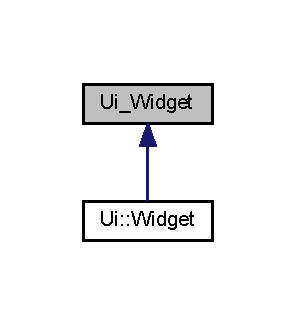
\includegraphics[width=142pt]{class_ui___widget__inherit__graph}
\end{center}
\end{figure}
\subsection*{Public Member Functions}
\begin{DoxyCompactItemize}
\item 
void \hyperlink{class_ui___widget_a9039ed8704971418cbe19ef8c9eea266}{setupUi} (QWidget $\ast$\hyperlink{class_widget}{Widget})
\item 
void \hyperlink{class_ui___widget_ae1cb85db8d3658df8dcd104361edcecb}{retranslateUi} (QWidget $\ast$\hyperlink{class_widget}{Widget})
\end{DoxyCompactItemize}
\subsection*{Public Attributes}
\begin{DoxyCompactItemize}
\item 
QLabel $\ast$ \hyperlink{class_ui___widget_a3126b93450dcc18cede73b9d1ee7c6b0}{label}
\item 
QLabel $\ast$ \hyperlink{class_ui___widget_a6f06b143349464b5b19ac0ffe2fc084d}{label\_2}
\item 
QLabel $\ast$ \hyperlink{class_ui___widget_adfcab5569ac08da197e14dba01390755}{label\_3}
\item 
QPushButton $\ast$ \hyperlink{class_ui___widget_a7dcf5da8902069415662905e93b0d5cb}{pushButton}
\item 
QLabel $\ast$ \hyperlink{class_ui___widget_a7d22bf9c5cf51754b1c145db5ca0da79}{label\_4}
\end{DoxyCompactItemize}


\subsection{Member Function Documentation}
\index{Ui\_Widget@{Ui\_Widget}!retranslateUi@{retranslateUi}}
\index{retranslateUi@{retranslateUi}!Ui\_Widget@{Ui\_Widget}}
\subsubsection[{\texorpdfstring{retranslateUi(QWidget $\ast$Widget)}{retranslateUi(QWidget *Widget)}}]{\setlength{\rightskip}{0pt plus 5cm}void Ui\_Widget::retranslateUi (
\begin{DoxyParamCaption}
\item[{QWidget $\ast$}]{Widget}
\end{DoxyParamCaption}
)\hspace{0.3cm}{\ttfamily [inline]}}\hypertarget{class_ui___widget_ae1cb85db8d3658df8dcd104361edcecb}{}\label{class_ui___widget_ae1cb85db8d3658df8dcd104361edcecb}


Here is the caller graph for this function:\nopagebreak
\begin{figure}[H]
\begin{center}
\leavevmode
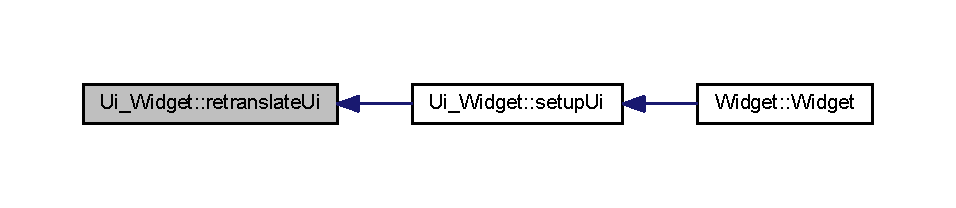
\includegraphics[width=350pt]{class_ui___widget_ae1cb85db8d3658df8dcd104361edcecb_icgraph}
\end{center}
\end{figure}


\index{Ui\_Widget@{Ui\_Widget}!setupUi@{setupUi}}
\index{setupUi@{setupUi}!Ui\_Widget@{Ui\_Widget}}
\subsubsection[{\texorpdfstring{setupUi(QWidget $\ast$Widget)}{setupUi(QWidget *Widget)}}]{\setlength{\rightskip}{0pt plus 5cm}void Ui\_Widget::setupUi (
\begin{DoxyParamCaption}
\item[{QWidget $\ast$}]{Widget}
\end{DoxyParamCaption}
)\hspace{0.3cm}{\ttfamily [inline]}}\hypertarget{class_ui___widget_a9039ed8704971418cbe19ef8c9eea266}{}\label{class_ui___widget_a9039ed8704971418cbe19ef8c9eea266}


Here is the call graph for this function:\nopagebreak
\begin{figure}[H]
\begin{center}
\leavevmode
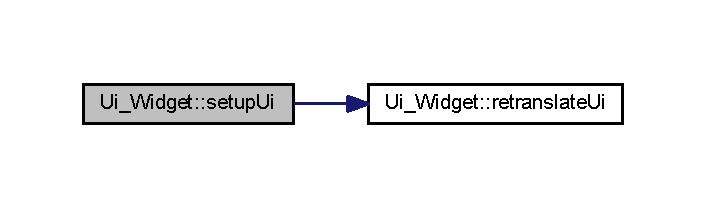
\includegraphics[width=339pt]{class_ui___widget_a9039ed8704971418cbe19ef8c9eea266_cgraph}
\end{center}
\end{figure}




Here is the caller graph for this function:\nopagebreak
\begin{figure}[H]
\begin{center}
\leavevmode
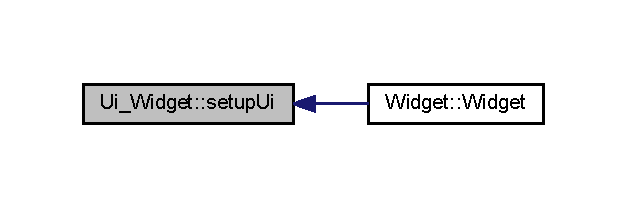
\includegraphics[width=301pt]{class_ui___widget_a9039ed8704971418cbe19ef8c9eea266_icgraph}
\end{center}
\end{figure}




\subsection{Member Data Documentation}
\index{Ui\_Widget@{Ui\_Widget}!label@{label}}
\index{label@{label}!Ui\_Widget@{Ui\_Widget}}
\subsubsection[{\texorpdfstring{label}{label}}]{\setlength{\rightskip}{0pt plus 5cm}QLabel$\ast$ Ui\_Widget::label}\hypertarget{class_ui___widget_a3126b93450dcc18cede73b9d1ee7c6b0}{}\label{class_ui___widget_a3126b93450dcc18cede73b9d1ee7c6b0}
\index{Ui\_Widget@{Ui\_Widget}!label\_2@{label\_2}}
\index{label\_2@{label\_2}!Ui\_Widget@{Ui\_Widget}}
\subsubsection[{\texorpdfstring{label\_2}{label_2}}]{\setlength{\rightskip}{0pt plus 5cm}QLabel$\ast$ Ui\_Widget::label\_2}\hypertarget{class_ui___widget_a6f06b143349464b5b19ac0ffe2fc084d}{}\label{class_ui___widget_a6f06b143349464b5b19ac0ffe2fc084d}
\index{Ui\_Widget@{Ui\_Widget}!label\_3@{label\_3}}
\index{label\_3@{label\_3}!Ui\_Widget@{Ui\_Widget}}
\subsubsection[{\texorpdfstring{label\_3}{label_3}}]{\setlength{\rightskip}{0pt plus 5cm}QLabel$\ast$ Ui\_Widget::label\_3}\hypertarget{class_ui___widget_adfcab5569ac08da197e14dba01390755}{}\label{class_ui___widget_adfcab5569ac08da197e14dba01390755}
\index{Ui\_Widget@{Ui\_Widget}!label\_4@{label\_4}}
\index{label\_4@{label\_4}!Ui\_Widget@{Ui\_Widget}}
\subsubsection[{\texorpdfstring{label\_4}{label_4}}]{\setlength{\rightskip}{0pt plus 5cm}QLabel$\ast$ Ui\_Widget::label\_4}\hypertarget{class_ui___widget_a7d22bf9c5cf51754b1c145db5ca0da79}{}\label{class_ui___widget_a7d22bf9c5cf51754b1c145db5ca0da79}
\index{Ui\_Widget@{Ui\_Widget}!pushButton@{pushButton}}
\index{pushButton@{pushButton}!Ui\_Widget@{Ui\_Widget}}
\subsubsection[{\texorpdfstring{pushButton}{pushButton}}]{\setlength{\rightskip}{0pt plus 5cm}QPushButton$\ast$ Ui\_Widget::pushButton}\hypertarget{class_ui___widget_a7dcf5da8902069415662905e93b0d5cb}{}\label{class_ui___widget_a7dcf5da8902069415662905e93b0d5cb}

\hypertarget{class_ui_1_1_widget}{}\section{Ui::Widget Class Reference}
\label{class_ui_1_1_widget}\index{Ui::Widget@{Ui::Widget}}


Inheritance diagram for Ui::Widget:\nopagebreak
\begin{figure}[H]
\begin{center}
\leavevmode
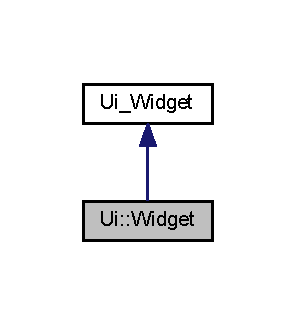
\includegraphics[width=142pt]{class_ui_1_1_widget__inherit__graph}
\end{center}
\end{figure}


Collaboration diagram for Ui::Widget:\nopagebreak
\begin{figure}[H]
\begin{center}
\leavevmode
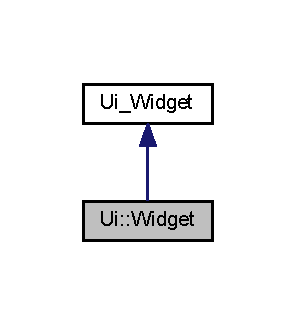
\includegraphics[width=142pt]{class_ui_1_1_widget__coll__graph}
\end{center}
\end{figure}
\subsection*{Additional Inherited Members}

\hypertarget{class_widget}{}\section{Widget Class Reference}
\label{class_widget}\index{Widget@{Widget}}


Inheritance diagram for Widget:\nopagebreak
\begin{figure}[H]
\begin{center}
\leavevmode
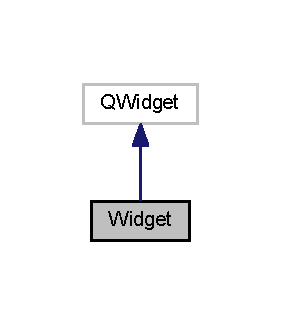
\includegraphics[width=135pt]{class_widget__inherit__graph}
\end{center}
\end{figure}


Collaboration diagram for Widget:
\nopagebreak
\begin{figure}[H]
\begin{center}
\leavevmode
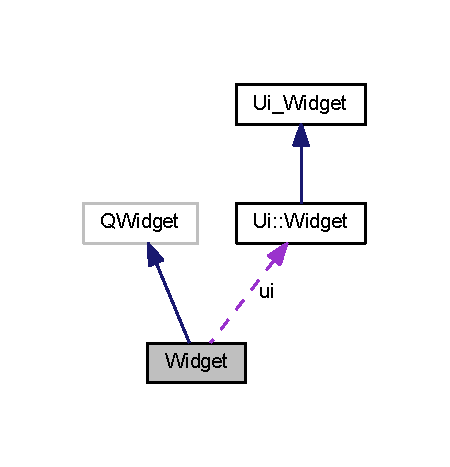
\includegraphics[width=216pt]{class_widget__coll__graph}
\end{center}
\end{figure}
\subsection*{Public Slots}
\begin{DoxyCompactItemize}
\item 
void \hyperlink{class_widget_adafcde4720aa7cb21f5d8966ae03c08c}{Print} ()
\end{DoxyCompactItemize}
\subsection*{Public Member Functions}
\begin{DoxyCompactItemize}
\item 
\hyperlink{class_widget_a29531c7f141e461322981b3b579d4590}{Widget} (QWidget $\ast$parent=0)
\item 
\hyperlink{class_widget_aa24f66bcbaaec6d458b0980e8c8eae65}{$\sim$Widget} ()
\end{DoxyCompactItemize}
\subsection*{Private Attributes}
\begin{DoxyCompactItemize}
\item 
\hyperlink{class_ui_1_1_widget}{Ui::Widget} $\ast$ \hyperlink{class_widget_a19c48cc897c43aa2e995fce9f7fb2418}{ui}
\end{DoxyCompactItemize}


\subsection{Constructor \& Destructor Documentation}
\index{Widget@{Widget}!Widget@{Widget}}
\index{Widget@{Widget}!Widget@{Widget}}
\subsubsection[{\texorpdfstring{Widget(QWidget $\ast$parent=0)}{Widget(QWidget *parent=0)}}]{\setlength{\rightskip}{0pt plus 5cm}Widget::Widget (
\begin{DoxyParamCaption}
\item[{QWidget $\ast$}]{parent = {\ttfamily 0}}
\end{DoxyParamCaption}
)\hspace{0.3cm}{\ttfamily [explicit]}}\hypertarget{class_widget_a29531c7f141e461322981b3b579d4590}{}\label{class_widget_a29531c7f141e461322981b3b579d4590}


Here is the call graph for this function:\nopagebreak
\begin{figure}[H]
\begin{center}
\leavevmode
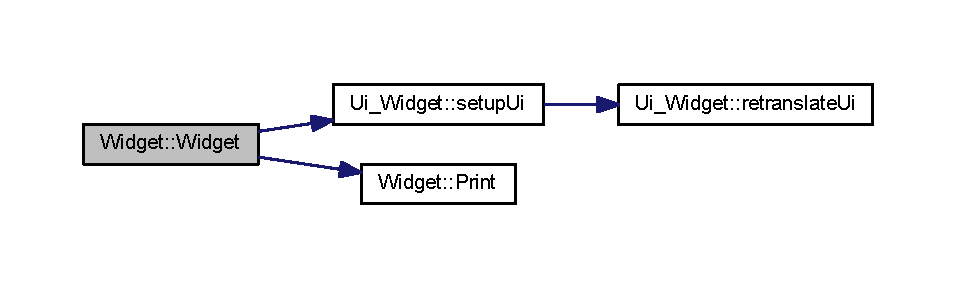
\includegraphics[width=350pt]{class_widget_a29531c7f141e461322981b3b579d4590_cgraph}
\end{center}
\end{figure}


\index{Widget@{Widget}!````~Widget@{$\sim$Widget}}
\index{````~Widget@{$\sim$Widget}!Widget@{Widget}}
\subsubsection[{\texorpdfstring{$\sim$Widget()}{~Widget()}}]{\setlength{\rightskip}{0pt plus 5cm}Widget::$\sim$Widget (
\begin{DoxyParamCaption}
{}
\end{DoxyParamCaption}
)}\hypertarget{class_widget_aa24f66bcbaaec6d458b0980e8c8eae65}{}\label{class_widget_aa24f66bcbaaec6d458b0980e8c8eae65}


\subsection{Member Function Documentation}
\index{Widget@{Widget}!Print@{Print}}
\index{Print@{Print}!Widget@{Widget}}
\subsubsection[{\texorpdfstring{Print}{Print}}]{\setlength{\rightskip}{0pt plus 5cm}void Widget::Print (
\begin{DoxyParamCaption}
{}
\end{DoxyParamCaption}
)\hspace{0.3cm}{\ttfamily [slot]}}\hypertarget{class_widget_adafcde4720aa7cb21f5d8966ae03c08c}{}\label{class_widget_adafcde4720aa7cb21f5d8966ae03c08c}


Here is the caller graph for this function:\nopagebreak
\begin{figure}[H]
\begin{center}
\leavevmode
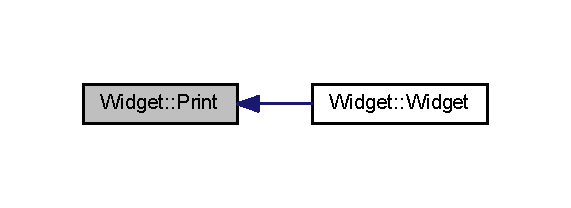
\includegraphics[width=274pt]{class_widget_adafcde4720aa7cb21f5d8966ae03c08c_icgraph}
\end{center}
\end{figure}




\subsection{Member Data Documentation}
\index{Widget@{Widget}!ui@{ui}}
\index{ui@{ui}!Widget@{Widget}}
\subsubsection[{\texorpdfstring{ui}{ui}}]{\setlength{\rightskip}{0pt plus 5cm}{\bf Ui::Widget}$\ast$ Widget::ui\hspace{0.3cm}{\ttfamily [private]}}\hypertarget{class_widget_a19c48cc897c43aa2e995fce9f7fb2418}{}\label{class_widget_a19c48cc897c43aa2e995fce9f7fb2418}

%--- End generated contents ---

% Index
\backmatter
\newpage
\phantomsection
\clearemptydoublepage
\addcontentsline{toc}{chapter}{Index}
\printindex

\end{document}
